\chapter{One-Dimensional Kinematics and Motion with Drag}
\label{ch:kinematics_1d}

\begin{chapterintro}
\textbf{Chapter Objectives:} In this chapter, we develop the differential and integral calculus of one-dimensional motion. You will master the inversion of acceleration functions $a(t)$, $a(v)$, and $a(x)$; read kinematic graphs; solve motion under linear and quadratic fluid resistance; derive terminal velocities; and prove why vertical projectiles spend more time descending than ascending.
\end{chapterintro}

\section{Fundamental Definitions of 1D Motion}

Consider a particle constrained to move along a straight line chosen as the $x$-axis.
\begin{itemize}[leftmargin=1.4em,itemsep=3pt]
  \item \textbf{Position}: $x(t) \in \mathbb{R}$ relative to origin $O$.
  \item \textbf{Displacement}: $\Delta x = x(t_2) - x(t_1)$.
  \item \textbf{Instantaneous Velocity}:
        \[
        \boxed{v(t) = \lim_{\Delta t\to 0}\frac{\Delta x}{\Delta t} = \frac{\dd x}{\dd t} = \dot{x}(t).}
        \]
  \item \textbf{Instantaneous Acceleration}:
        \[
        \boxed{a(t) = \lim_{\Delta t\to 0}\frac{\Delta v}{\Delta t} = \frac{\dd v}{\dd t} = \frac{\dd^2 x}{\dd t^2} = \ddot{x}(t).}
        \]
\end{itemize}

\begin{figure}[htbp]
\centering
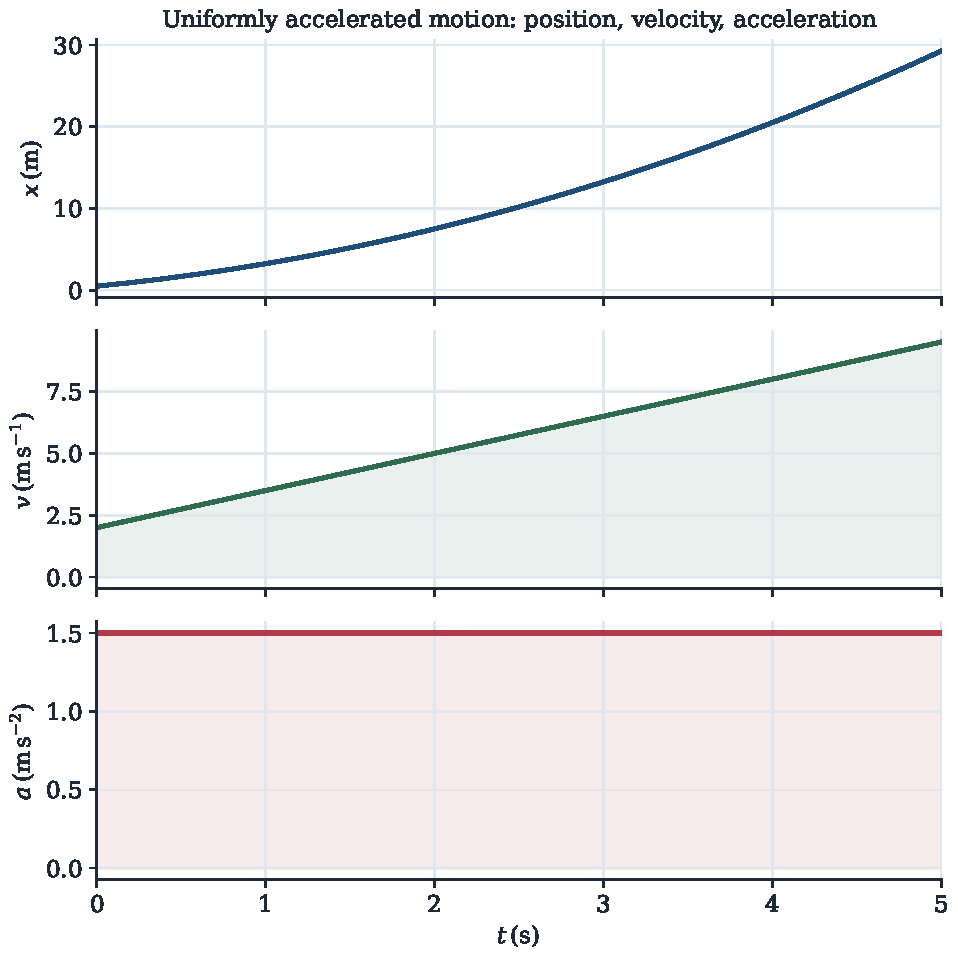
\includegraphics[width=0.88\textwidth]{figures/05_motion_graphs.pdf}
\caption{Kinematic graphs in 1D. The velocity is the slope of $x(t)$; the displacement is the area under $v(t)$; the acceleration is the slope of $v(t)$.}
\label{fig:motion_graphs}
\end{figure}

\section{The Three Standard Integration Protocols}

In general physical problems, acceleration is not constant but depends on time $t$, velocity $v$, or position $x$:

\begin{center}
\renewcommand{\arraystretch}{1.4}
\begin{tabular}{@{}lll@{}}
\toprule
\textbf{Given Acceleration} & \textbf{Separation of Variables} & \textbf{Integral Formula} \\
\midrule
$a = a(t)$ & $\dd v = a(t)\,\dd t$ & $v(t) = v_0 + \int_0^t a(t')\,\dd t'$ \\
$a = a(v)$ & $\dd t = \frac{\dd v}{a(v)}, \quad \dd x = \frac{v\,\dd v}{a(v)}$ & $t(v) = \int_{v_0}^v \frac{\dd v'}{a(v')}, \quad x(v) = x_0 + \int_{v_0}^v \frac{v'\,\dd v'}{a(v')}$ \\
$a = a(x)$ & $v\,\dd v = a(x)\,\dd x$ & $v^2(x) = v_0^2 + 2\int_{x_0}^x a(x')\,\dd x'$ \\
\bottomrule
\end{tabular}
\end{center}

\begin{lawbox}{The Chain Rule Identity for Acceleration}
By the chain rule:
\[
\boxed{a = \frac{\dd v}{\dd t} = \frac{\dd v}{\dd x}\frac{\dd x}{\dd t} = v\frac{\dd v}{\dd x} = \frac{\dd}{\dd x}\left(\frac{1}{2}v^2\right).}
\]
This timeless relation connects acceleration directly to spatial displacement without reference to time.
\end{lawbox}

\section{Motion with Fluid Resistance}

\begin{figure}[htbp]
\centering
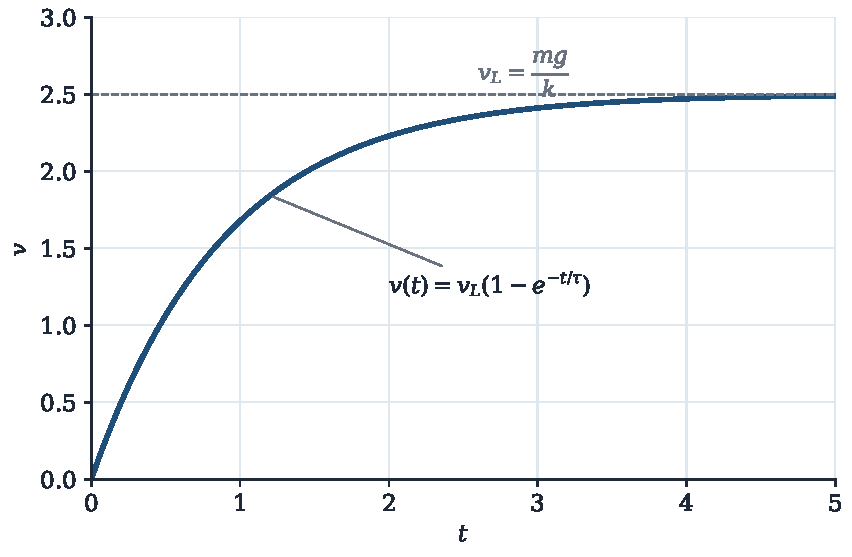
\includegraphics[width=0.74\textwidth]{figures/19_terminal_velocity.pdf}
\caption{Vertical fall under gravity with drag. The velocity asymptotically approaches terminal velocity $v_t$ where drag balances weight.}
\label{fig:terminal_velocity}
\end{figure}

When a body moves through a fluid, it experiences a resistive drag force opposing its velocity:
\begin{itemize}[leftmargin=1.4em,itemsep=3pt]
  \item \textbf{Linear (Stokes) Drag} ($F_d = -b v$): Operates at low velocities and tiny scales (pollen grains, mist droplets, oil droplets in Millikan's experiment).
  \item \textbf{Quadratic (Newton) Drag} ($F_d = -c v^2$): Operates at macroscopic scales and everyday speeds (baseballs, skydivers, automobiles, airplanes).
\end{itemize}

\section{Extensive Worked Examples}

\begin{workedexample}{Vertical Fall with Linear Drag (Exact Solution)}
A particle of mass $m$ is released from rest at $t = 0$ in a gravitational field $g$ subject to a linear viscous drag force $F_d = -b v$.
(a) Write the differential equation of motion and identify the characteristic velocity $v_t$ and time scale $\tau$.
(b) Solve for the instantaneous velocity $v(t)$.
(c) Integrate $v(t)$ to obtain the position $z(t)$.
(d) Examine the short-time ($t \ll \tau$) and long-time ($t \gg \tau$) limits.

\paragraph{Solution.}

(a) Orient the vertical $z$-axis downward, so gravity is $+mg$ and drag is $-bv$.
Newton's second law:
\[
m\frac{\dd v}{\dd t} = mg - bv \implies \frac{\dd v}{\dd t} = g - \frac{b}{m}v = -\frac{b}{m}\left(v - \frac{mg}{b}\right).
\]
Define the \textbf{characteristic time constant} $\tau$ and \textbf{terminal velocity} $v_t$:
\[
\boxed{\tau = \frac{m}{b}}, \qquad \boxed{v_t = \frac{mg}{b} = g\tau.}
\]
Then the equation becomes:
\[
\frac{\dd v}{\dd t} = -\frac{1}{\tau}(v - v_t).
\]

(b) Separating variables:
\[
\frac{\dd v}{v - v_t} = -\frac{\dd t}{\tau}.
\]
Integrating with initial condition $v(0) = 0$:
\[
\int_0^v \frac{\dd v'}{v' - v_t} = -\frac{1}{\tau}\int_0^t \dd t' \implies \ln\left(\frac{v - v_t}{-v_t}\right) = -\frac{t}{\tau} \implies 1 - \frac{v}{v_t} = e^{-t/\tau}.
\]
Solving for $v(t)$:
\[
\boxed{v(t) = v_t\left(1 - e^{-t/\tau}\right).}
\]

(c) Integrating $v(t) = \frac{\dd z}{\dd t}$ with $z(0) = 0$:
\[
z(t) = \int_0^t v_t\left(1 - e^{-t'/\tau}\right)\dd t' = v_t\left[ t' + \tau e^{-t'/\tau} \right]_0^t = \boxed{v_t t - v_t\tau\left(1 - e^{-t/\tau}\right).}
\]

(d) \textbf{Asymptotic limits:}
\begin{itemize}[leftmargin=1.4em,itemsep=2pt]
  \item \textbf{Short-time limit ($t \ll \tau$)}: Expand the exponential $e^{-t/\tau} \approx 1 - \frac{t}{\tau} + \frac{t^2}{2\tau^2}$:
  \[
  v(t) = v_t\left[ 1 - \left(1 - \frac{t}{\tau} + \frac{t^2}{2\tau^2}\right) \right] \approx v_t\frac{t}{\tau} = (g\tau)\frac{t}{\tau} = gt.
  \]
  \[
  z(t) \approx v_t t - v_t\tau\left[ \frac{t}{\tau} - \frac{t^2}{2\tau^2} \right] = v_t t - v_t t + \frac{1}{2}\frac{v_t}{\tau}t^2 = \frac{1}{2}gt^2.
  \]
  At initial times, drag is negligible, recovering pure vacuum free fall!
  \item \textbf{Long-time limit ($t \gg \tau$)}: The exponential term decays to zero ($e^{-t/\tau} \to 0$):
  \[
  v(t) \to v_t = \text{const}, \qquad z(t) \to v_t t - v_t\tau.
  \]
  The particle moves at constant terminal velocity $v_t$, with a spatial delay $v_t\tau$ representing the initial acceleration phase.
\end{itemize}
\end{workedexample}

\begin{workedexample}{Vertical Fall with Quadratic Drag (Hyperbolic Solution)}
A skydiver of mass $m$ falls from rest under quadratic aerodynamic drag $F_d = -c v^2$.
(a) Determine the terminal velocity $v_t$.
(b) Integrate the equation of motion using separation of variables to show:
\[
v(t) = v_t\tanh\left(\frac{gt}{v_t}\right).
\]
(c) Find the distance fallen $z(t)$ and the timeless relation $v(z)$.

\paragraph{Solution.}

(a) Downward equation of motion:
\[
m\frac{\dd v}{\dd t} = mg - cv^2.
\]
At terminal velocity, acceleration vanishes:
\[
mg - cv_t^2 = 0 \implies \boxed{v_t = \sqrt{\frac{mg}{c}}.}
\]
Rewriting the equation of motion using $c/m = g/v_t^2$:
\[
\frac{\dd v}{\dd t} = g\left(1 - \frac{v^2}{v_t^2}\right).
\]

(b) Separating variables:
\[
\frac{\dd v}{1 - (v/v_t)^2} = g\,\dd t.
\]
Using the standard integral $\int \frac{\dd u}{1 - u^2} = \operatorname{artanh}(u)$:
\[
v_t\int_0^{v/v_t} \frac{\dd u}{1 - u^2} = gt \implies v_t\operatorname{artanh}\left(\frac{v}{v_t}\right) = gt.
\]
Taking the hyperbolic tangent of both sides:
\[
\boxed{v(t) = v_t\tanh\left(\frac{gt}{v_t}\right).}
\]
Since $\tanh(x) \to 1$ as $x \to \infty$, the speed smoothly approaches $v_t$. At $t = 2v_t/g$, $\tanh(2) \approx 0.964$: the skydiver reaches over $96\%$ of terminal velocity in roughly two time constants.

(c) Distance fallen:
\[
z(t) = \int_0^t v(t')\dd t' = v_t\int_0^t \tanh\left(\frac{gt'}{v_t}\right)\dd t'.
\]
Using $\int \tanh(ax)\dd x = \frac{1}{a}\ln\cosh(ax)$:
\[
\boxed{z(t) = \frac{v_t^2}{g}\ln\cosh\left(\frac{gt}{v_t}\right).}
\]
For the spatial relation $v(z)$, use $v\frac{\dd v}{\dd z} = g\left(1 - \frac{v^2}{v_t^2}\right)$:
\[
\frac{v\,\dd v}{1 - v^2/v_t^2} = g\,\dd z.
\]
Let $w = 1 - v^2/v_t^2 \implies \dd w = -\frac{2v}{v_t^2}\dd v$:
\[
-\frac{v_t^2}{2}\int_1^{1 - v^2/v_t^2} \frac{\dd w}{w} = gz \implies -\frac{v_t^2}{2}\ln\left(1 - \frac{v^2}{v_t^2}\right) = gz.
\]
Exponentiating:
\[
1 - \frac{v^2}{v_t^2} = e^{-2gz/v_t^2} \implies \boxed{v(z) = v_t\sqrt{1 - e^{-2gz/v_t^2}}.}
\]
\end{workedexample}

\begin{workedexample}{Asymmetry of Ascent and Descent under Quadratic Drag}
A projectile is fired vertically upward with initial speed $v_0$ in air with quadratic drag $c v^2$.
(a) Find the maximum height $H$ reached by the projectile.
(b) Find the time of ascent $t_{\text{up}}$.
(c) The projectile falls back down from height $H$ to the ground. Find its landing speed $v_{\text{land}}$ and time of descent $t_{\text{down}}$.
(d) Prove that $t_{\text{down}} > t_{\text{up}}$: the projectile always spends more time coming down than going up!

\paragraph{Solution.}

(a) During ascent (upward $y$-axis): both gravity and drag point downward:
\[
m\frac{\dd v}{\dd t} = -mg - cv^2 = -mg\left(1 + \frac{v^2}{v_t^2}\right).
\]
Using $v\frac{\dd v}{\dd y} = -g\left(1 + \frac{v^2}{v_t^2}\right)$ from $(y=0, v=v_0)$ to $(y=H, v=0)$:
\[
\int_{v_0}^0 \frac{v\,\dd v}{1 + v^2/v_t^2} = -g\int_0^H \dd y \implies \left[ \frac{v_t^2}{2}\ln\left(1 + \frac{v^2}{v_t^2}\right) \right]_{v_0}^0 = -gH.
\]
\[
-\frac{v_t^2}{2}\ln\left(1 + \frac{v_0^2}{v_t^2}\right) = -gH \implies \boxed{H = \frac{v_t^2}{2g}\ln\left(1 + \frac{v_0^2}{v_t^2}\right).}
\]

(b) For time of ascent:
\[
\frac{\dd v}{\dd t} = -g\left(1 + \frac{v^2}{v_t^2}\right) \implies \int_{v_0}^0 \frac{\dd v}{1 + (v/v_t)^2} = -g\int_0^{t_{\text{up}}}\dd t.
\]
Using $\int \frac{\dd u}{1 + u^2} = \arctan(u)$:
\[
v_t\left[ 0 - \arctan\left(\frac{v_0}{v_t}\right) \right] = -gt_{\text{up}} \implies \boxed{t_{\text{up}} = \frac{v_t}{g}\arctan\left(\frac{v_0}{v_t}\right).}
\]

(c) During descent from rest at height $H$:
From Example 3.2, the landing speed satisfies $v_{\text{land}} = v_t\sqrt{1 - e^{-2gH/v_t^2}}$.
Substitute $e^{-2gH/v_t^2} = \frac{1}{1 + v_0^2/v_t^2}$:
\[
v_{\text{land}} = v_t\sqrt{1 - \frac{1}{1 + v_0^2/v_t^2}} = v_t\sqrt{\frac{v_0^2/v_t^2}{1 + v_0^2/v_t^2}} = \boxed{\frac{v_0}{\sqrt{1 + v_0^2/v_t^2}} < v_0.}
\]
The landing speed is strictly smaller than the launch speed due to dissipated mechanical energy!
For descent time, from $v(t) = v_t\tanh(gt/v_t)$:
\[
\tanh\left(\frac{gt_{\text{down}}}{v_t}\right) = \frac{v_{\text{land}}}{v_t} = \frac{v_0/v_t}{\sqrt{1 + v_0^2/v_t^2}}.
\]
Using the identity $\operatorname{artanh}\left(\frac{x}{\sqrt{1+x^2}}\right) = \operatorname{arsinh}(x)$:
\[
\boxed{t_{\text{down}} = \frac{v_t}{g}\operatorname{arsinh}\left(\frac{v_0}{v_t}\right).}
\]

(d) To compare $t_{\text{up}}$ and $t_{\text{down}}$, define $\xi = v_0/v_t > 0$:
\[
t_{\text{up}} = \frac{v_t}{g}\arctan(\xi), \qquad t_{\text{down}} = \frac{v_t}{g}\operatorname{arsinh}(\xi).
\]
For any $\xi > 0$, we have:
\[
\operatorname{arsinh}(\xi) = \ln\left(\xi + \sqrt{1+\xi^2}\right) > \arctan(\xi).
\]
(Indeed, $\frac{\dd}{\dd\xi}\operatorname{arsinh}\xi = \frac{1}{\sqrt{1+\xi^2}} > \frac{1}{1+\xi^2} = \frac{\dd}{\dd\xi}\arctan\xi$ for all $\xi > 0$, and both are zero at $\xi=0$).
Therefore:
\[
\boxed{t_{\text{down}} > t_{\text{up}}.}
\]
The projectile \textbf{always takes longer to fall down than to rise}!
On the way up, gravity and drag cooperate (both pull downward, producing large decelerations $> g$). On the way down, drag opposes gravity (deceleration is $< g$). Consequently, average speed during descent is lower, requiring a longer transit time.
\end{workedexample}
